\chapter{Arkitektur Worksheet}
Arkitekturen er opbygget af fire komponenter: \textit{manager}, \textit{moduler}, \textit{DB access} og \textit{DB}.
En skitse af arkitekturen kan ses på \cref{arkitektur_udkast_1}.
\begin{figure}[h]
	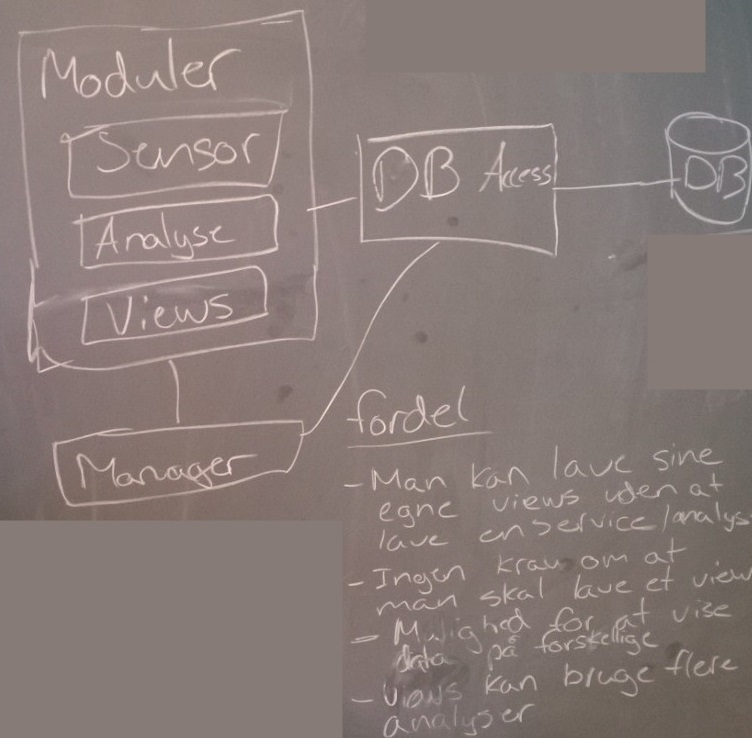
\includegraphics[width=\textwidth]{architecture_draft}
	\label{arkitektur_udkast_1}
	\caption{Første udkast til arkitektur.}
\end{figure}

\subsection*{Manager}
Denne komponent står for at holde styr på hvilke moduler der er installeret og opretter tabeller i databasen for dem.
\textit{Manageren} indeholder også et GUI så brugeren kan tilføje og fjerne moduler.
\textit{Manageren} har også logikken for hvilke \textit{analyse} moduler der kan vises i hvilke \textit{views}.
Desuden indeholder \textit{manageren} også et JSON skema for hver modul-type i \textit{moduler} komponenten.
\stefan{et eller flere skemaer? Muligvis har views anderledes skema, men analyse og sensorer har det samme}

\subsection*{Moduler}
Denne komponent består af tre konceptuelle lag: \textit{sensor}, \textit{analyse} og \textit{views}.
Alle moduler indeholder en modulbeskrivelse som beskrevet i \cref{modul_definition}. 
Alle moduler kan skrive til deres egne tabeller i databasen, samt læse fra alle andre modulers tabeller.

\stefan{skal der være eksempler på sensorer, moduler, etc?}
\paragraph{Sensor} \textit{Sensor}laget indeholder alle de moduler der logger data fra sensorer eller logger data fra applikationer.

\paragraph{Analyse}
\textit{Analyse}laget indeholder alle moduler der bruger et antal \textit{sensor}moduler og analyserer det data for derefter at gemme det i en databasetabel.

\paragraph{Views}
\textit{Views}laget indeholder alle moduler der gør det muligt at visualisere de analyserede data.
Den angiver hvilke og hvor mange datatyper den kan vise.

\subsection*{DB Access}
Denne komponent styrer adgangen til databasen så det sker på en ensrettet måde.
DB Access holder derudover styr på hvem der må skrive og læse fra de enkelte tabeller.

\subsection*{DB}
Til dette projekt er valgt en sqlite database da denne er standard i android.

\section*{Arkitekturens styrker}
Denne modulbaserede arkitektur har \textit{moduler}komponenten som indeholder forskellige moduler.
Disse moduler kan kombineres hvilket er en fordel da det giver mulighed for at tilføje flere moduler løbende.
Det giver mulighed for at et view kan bruges til at vise mange forskellige analyser og at analyser man vises af mange forskellige views.

Da smartphones udvikler sig hele tiden og sikkert får en del nye sensorer i fremtiden er det ikke et problem, fordi det er muligt at tilføje et nyt sensor modul.

\textbf{Det har ikke været muligt at finde et umiddelbart arkitektur-mønster for dette.}
\stefan{vi bør nok udvide dette, det virker lidt tyndt at skrive}